%!TEX root = /Users/louis/Documents/PhD/Deliverables/Thesis/thesis.tex

\section{Metamodel-Independent Syntax}
\label{sec:mmi_syntax}
Section~\ref{subsec:modelling_framework_characteristics} discussed the way in which modelling frameworks implicitly enforce conformance, and hence prevent the loading of non-conformant models. Additionally, modelling frameworks provide little support for checking the conformance of a model with other versions of a metamodel, which is potentially useful during metamodel installation. In Section~\ref{sec:requirements_identification}, these concerns lead to the identification of the following requirement: \emph{This thesis must investigate the extension of existing modelling frameworks to support the loading of non-conformant models and conformance checking of models against other metamodels.}

This section describes the way in which existing modelling frameworks load and store models using a metamodel-specific syntax, proposes an alternative syntax and demonstrates how this facilitates automatic consistency checking. The work presented in this section has been published in \cite{rose09enhanced}.

% TODO - intro example
% TODO - consistent formatting of metamodel elements and model elements
% TODO - present MM independent syntax. Make clear that it is an ABSTRACT syntax.


\subsection{Binding to a specific metamodel}
\label{subsec:binding_specific}
XMI (Section~\ref{}) is the canonical model storage representation used by many contemporary modelling frameworks. Because models and metamodels are kept separate (Section~\ref{subsec:modelling_framework_characteristics}), XMI provides a mechanism for referring to metamodel types from a model. In the preamble of an XMI document, metamodels are imported using namespaces. In the body of an XMI document, namespaces are used to refer to metamodel types. In Listing~\ref{lst:xmi}, line 2 imports two metamodels to the namespaces \texttt{xmi} and \texttt{families}. The former is used to reference types provided by the modelling framework, and the latter to reference types provided by the metamodel in Figure~\ref{fig:x}.

Modelling frameworks bind a model to its metamodel using the underlying programming language (Section~\ref{subsec:modelling_framework_characteristics}). The metamodel defines the way in which model elements will be bound, and binding is often strongly-typed: each metamodel type is mapped to a corresponding type in the underlying programming language. The XMI in Listing~\ref{lst:xmi} contains three \texttt{Person}s, Franz (line 3), Julie (line 4) and Hermann (line 5). Line 3 indicates that Julie is the mother and Hermann is the father of Franz. The mothers and fathers of Julie and Hermann are not specified. Each person defines an XMI ID (a universally unique identifier), and a name. The IDs are used for inter-element references, such as for the values of the mother and father features.

\begin{lstlisting}[caption=Person model in XMI, label=lst:xmi, language=XML]
<?xml version="1.0" encoding="ASCII"?>
<xmi:XMI xmi:version="2.0" xmlns:xmi="http://www.omg.org/XMI" xmlns:families="http://www.cs.york.ac.uk/families">
	<families:Person xmi:id="_xNSb8KfZEd,0dNl1iq3EdQ" name="Franz" mother="_6ef33ff010b31df8a39080" father="_F520cDaa0jN,i10s8xZp2a" />
	<families:Person xmi:id="_6ef33ff010b31df8a39080" name="Julie" />
	<families:Person xmi:id="_F520cDaa0jN,i10s8xZp2a" name="Hermann" />
</xmi:XMI>
\end{lstlisting}

Binding a model element involves instantiating, in the underlying programming language, the metamodel type, and populating the attributes of the instantiated object with values that correspond to those specified in the model. Figure~\ref{fig:y} shows the (Java) objects that would be created by EMF when loading the XMI in Listing~\ref{lst:xmi}.

When a metamodel changes, existing models might reference types and features that no longer exist, and, hence, binding fails when a model does not conform to its metamodel. For example, suppose that the mother and father reference are removed from the metamodel in Figure~\ref{fig:x}, and are replaced by a unifying parents reference. Binding (i.e. constructing the objects in Figure~\ref{fig:y}) would now fail, as the Person class does not define mother and father features. XMI refers to metamodel types and features by name, and, hence, binding can fail following metamodel evolution.

\subsection{Binding to a generic metamodel}
\label{subsec:binding}
For situations when a model does not conform to its metamodel, this thesis proposes an alternative to the binding mechanism described in Section~\ref{subsec:binding_specific}, which binds a model to a \emph{generic} metamodel. A generic metamodel reflects the characteristics of the metamodelling language and consequently every model conforms to the generic metamodel. Figure~\ref{fig:slot_model} shows a minimal generic metamodel for MOF, which is based on the MOF metamodel \cite{mof}. Model elements are bound to \texttt{Object}, data values to \texttt{Slot}.

\begin{figure}[htbp]
  \centering
  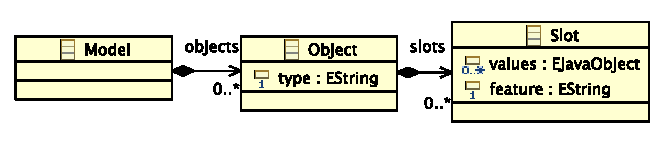
\includegraphics[width=3.3in]{5.Implementation/slot_model.pdf}
  \caption[A generic metamodel for MOF]{A generic metamodel for MOF, based on \cite{MOF} and taken from \cite{rose09enhanced}.}
  \label{fig:slot_model}
\end{figure}

Using the metamodel in Figure~\ref{fig:slot_model} in conjunction with MOF, conformance constraints can be expressed, as shown below. A minimal subset of MOF is shown in Figure~\ref{fig:minimal_mof}.

\begin{figure}[htbp]
  \centering
  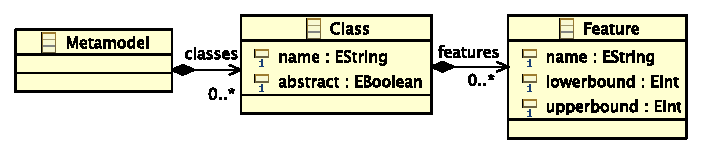
\includegraphics[width=3.3in]{5.Implementation/mof.pdf}
  \caption[Minimal MOF metamodel]{Minimal MOF metamodel, based on \cite{MOF} and taken from \cite{rose09enhanced}.}
  \label{fig:minimal_mof}
\end{figure}

The following constraints between metamodels (e.g. instances of MOF, Figure~\ref{fig:minimal_mof}) and models represented with a generic metamodel (e.g. instances of Figure~\ref{fig:slot_model}) can be used to express conformance:

\begin{enumerate}
	\item Each object's type must be the name of some non-abstract metamodel class.
	\item Each object must specify a slot for each mandatory feature of its type.
	\item Each slot's feature must be the name of a metamodel feature. That metamodel feature must belong to the slot's owning object's type.
	\item Each slot must be multiplicity-compatible with its feature. More specifically, each slot must contain at least as many values as its feature's lower bound, and at most as many values as its feature's upper bound.
  \item Each slot must be type-compatible with its feature.
\end{enumerate}

% TODO illustrate for person (think I do this in the next section, maybe move to here)

The way in which type-compatibility is checked depends on the way in which the modelling framework is implemented. In EMF, for example, model values conform either to types defined in a metamodel, or to types defined in the underlying programming language, Java. EMF provides programmatic access to a metamodel's type system, which can be used to implement type-compatibility checks.

Conformance constraints vary over modelling languages. For example, Ecore, the modelling language of EMF, is similar to but not the same as MOF. Metamodel features defined in Ecore can be marked as transient (not stored to disk) or unchangeable (read-only). Consequently in EMF, conformance constraints are required to restrict the feature value of slots to only non-transient, changeable features.


\subsection{Example}
\label{subsec:mmi_syntax_example}
By binding a model to the generic metamodel presented in Figure~\ref{fig:slot_model} rather than to the underlying programming languages types defined in its metamodel, conformance can be checked using the above constraints. Binding the XMI in Listing~\ref{lst:xmi} to the generic metamodel shown in Figure~\ref{fig:slot_model} produces three instances of Object, illustrated as a UML object diagram in Figure~\ref{fig:generic_binding}. For clarity, instances of Object are shaded, and instances of Slot are unshaded. Each of the three Objects, has a slot whose feature is ``name''. The value of each slot varies: one has the value ``Franz'', another has the value ``Julie'' and another has the value ``Hermann''. The object containing the slot with value ``Franz'' contains two further slots: one whose feature is ``mother'' and whose value is a reference to the object that contains the name slot with the value ``Julie''\footnote{Reference values in the generic metamodel are implemented using the proxy design pattern \cite{gamma95patterns}.} and one whose feature is ``father'' and whose value is a reference to the object containing ``Hermann''. 

\begin{figure}[htbp]
  \centering
  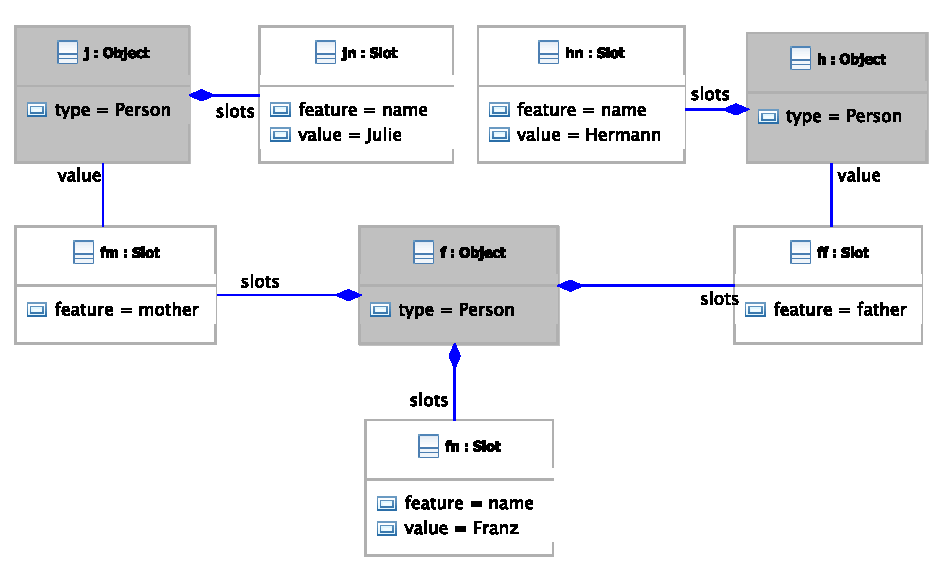
\includegraphics[width=4in]{5.Implementation/GenericBinding.pdf}
  \caption{Exemplar instantiation of generic metamodel.}
  \label{fig:generic_binding}
\end{figure}

After binding to the generic metamodel, the conformance of a model can be checked against any specific metamodel. To illustrate the value of the generic metamodel, consider what happens when the specific metamodel evolves. The mother and father references have been removed, and replaced by a unifying parents reference. Conformance checking for the object representing Franz would now fail because it defines slots for features ``mother'' and ``father'', which are no longer defined for the metamodel class ``Person''. Specifically, the model element representing Franz does not satisfy conformance constraint 4 (Section~\ref{subsec:binding}), which states: \emph{each slot's feature must be the name of a metamodel feature. That metamodel feature must belong to the slot's owning object's type}. 

\subsection{Structures built atop the metamodel-independent syntax}
There are many potential uses for the metamodel-independent syntax described in this section. Section~\ref{sec:notation} describes a textual modelling notation integrated with the metamodel-independent syntax to achieve live conformance checking. The migration language presented in Section~\ref{sec:flock} can be used with the metamodel independent syntax to perform partial migration (i.e. to produce models that conform to a generic metamodel rather than their evolved metamodel), but implementation of this work is not complete\footnote{The current version does not support metamodels that contain non-containment references and enumeration types.}.

One of the model migration tools discussed in Section~\ref{sec:analyis_of_languages_used_for_migration}, COPE \cite{herrmannsdoerfer09cope}, uses a metamodel-independent syntax similar to the one presented in this section. The metamodel-independent syntax presented here was developed independently of the metamodel-independent syntax developed for COPE. The two syntaxes were first published in 2008 (\cite{rose08hutn,herrmannsdoerfer08cope}), and are both conceptually similar to the metamodel for UML Object diagrams \cite{uml14}.

In addition to these uses, the metamodel-independent syntax is potentially useful during metamodel installation. As discussed in Section~\ref{subsec:modelling_framework_characteristics}, metamodel developers do not have access to downstream models, and conformance is implicitly enforced by modelling frameworks. Consequently, the conformance of models may be affected by the installation of a new version of a metamodel, and the conformance of models cannot be checked during installation. Typically, installing a new version of a metamodel can result in models that no longer conform to their metamodel and cannot be used with the modelling framework. Moreover, a user discovers conformance problems only when attempting to use a model after installation has completed, and not as part of the installation process.

% TODO - Consider discussing the number of revisions of say, UML (and other metamodels), in Chapter 2. This will allow the reader to get a sense of the scale of the problem.

To enable conformance checking as part of metamodel installation in EMF, the metamodel-independent syntax has been integrated with Concordance in \cite{rose10concordance}. Concordance provides a mechanism for resolving inter-model references (such as those between models and their metamodels), and can be used to efficiently determine the instances of a metamodel. Without Concordance, determining the the instances of a metamodel is possible only by checking every model in the workspace.

Integrating Concordance and the metamodel-independent syntax resulted in a service, executed after the installation of a metamodel, which identifies the models that are affected by the metamodel changes. All models that conform to the old version of the metamodel are checked for conformance with the new metamodel. As such, conformance checking occurs automatically and immediately after metamodel installation. Conformance problems are detected and reported immediately, rather than when the user next attempts to load an affected model.


\subsubsection{Summary}
Modelling frameworks implicitly enforce conformance, which presents challenges for managing co-evolution. In particular, detecting and reconciling conformance problems involves managing non-conformant models, which cannot be loaded by modelling frameworks and hence cannot be used with model editors or model management operations. The metamodel-independent syntax proposed in this section enables modelling frameworks to load non-conformant models by binding models to a generic metamodel. The metamodel-independent syntax has been integrated with Concordance \cite{rose10concordance} to facilitate the reporting of conformance problems during metamodel installation, and underpins the implementation of the textual modelling notation presented in Sections~\ref{sec:notation}. The benefits and drawbacks of the metamodel-independent syntax in the context of user-driven co-evolution are explored in Chapter~\ref{Evaluation}. 
